%%%%%%%%%%%%%%%%%%%%%%%%%%%%%%%%%%%%%%%%%%%%%%%%%%%%%%%%%%%%%%%%%%%%%%%%%%%%%%%%
%2345678901234567890123456789012345678901234567890123456789012345678901234567890
%        1         2         3         4         5         6         7         8

\documentclass[letterpaper, 10 pt, conference]{ieeeconf}  % Comment this line out if you need a4paper

%\documentclass[a4paper, 10pt, conference]{ieeeconf}      % Use this line for a4 paper

\IEEEoverridecommandlockouts                              % This command is only needed if 
                                                          % you want to use the \thanks command

\overrideIEEEmargins                                      % Needed to meet printer requirements.

%In case you encounter the following error:
%Error 1010 The PDF file may be corrupt (unable to open PDF file) OR
%Error 1000 An error occurred while parsing a contents stream. Unable to analyze the PDF file.
%This is a known problem with pdfLaTeX conversion filter. The file cannot be opened with acrobat reader
%Please use one of the alternatives below to circumvent this error by uncommenting one or the other
%\pdfobjcompresslevel=0
%\pdfminorversion=4

% See the \addtolength command later in the file to balance the column lengths
% on the last page of the document

% The following packages can be found on http:\\www.ctan.org
%\usepackage{graphics} % for pdf, bitmapped graphics files
%\usepackage{epsfig} % for postscript graphics files
%\usepackage{mathptmx} % assumes new font selection scheme installed
%\usepackage{times} % assumes new font selection scheme installed
%\usepackage{amsmath} % assumes amsmath package installed
%\usepackage{amssymb}  % assumes amsmath package installed
\usepackage{times}
\usepackage{epsfig}
\usepackage{graphicx}
\usepackage{amsmath}
\usepackage{amssymb}
\usepackage{xspace}
\usepackage{multirow}
\usepackage{comment}
\usepackage{color}
\usepackage{textcomp}
\usepackage{subcaption}
\captionsetup{compatibility=false}
\usepackage{tabulary}
\usepackage{epigraph}
\usepackage[table]{xcolor}
\definecolor{grey}{rgb}{0.9,0.9,0.9}
\usepackage{ctable}
\usepackage{algorithm}
\usepackage{algorithmic}
\usepackage{wrapfig}
\usepackage[pagebackref=true,breaklinks=true,colorlinks,bookmarks=false]{hyperref}

\makeatletter
\DeclareRobustCommand\onedot{\futurelet\@let@token\@onedot}
\def\@onedot{\ifx\@let@token.\else.\null\fi\xspace}

\def\eg{\emph{e.g}\onedot} \def\Eg{\emph{E.g}\onedot}
\def\ie{\emph{i.e}\onedot} \def\Ie{\emph{I.e}\onedot}
\def\cf{\emph{c.f}\onedot} \def\Cf{\emph{C.f}\onedot}
\def\aka{a.k.a\onedot} \def\Aka{A.k.a\onedot}
\def\etc{\emph{etc}\onedot} \def\vs{\emph{vs}\onedot}
\def\wrt{w.r.t\onedot} \def\dof{d.o.f\onedot}
\def\etal{\emph{et al}\onedot}
\makeatother

\DeclareMathOperator{\bool}{bool}
\newcommand{\G}{\mathcal{G}}
\newcommand{\E}{\mathcal{E}}
\newcommand{\B}{\mathcal{B}}
\newcommand{\ROI}{\textit{LaneRoI} }
\newcommand{\RCNN}{\textbf{LaneRCNN} }


\title{\LARGE \bf
LaneRCNN: Distributed Representations for Graph-Centric Motion Forecasting
}

\author{
  Wenyuan Zeng$^{1}$\quad Ming Liang \quad Renjie Liao$^{1}$ \quad
  Raquel Urtasun$^{1}$%
  % \thanks{$^1$ University of Toronto.}
  \thanks{$^{1}$ {Univ of Toronto. Correspondence}:
\texttt{wenyuan@cs.toronto.edu}, \texttt{urtasun@cs.toronto.edu}}%
    % , \small\texttt{\{wenyuan, rjliao,
  % urtasun\}@cs.toronto.edu}}
}
 % \small\texttt{\{wenyuan, rjliao, urtasun\}@cs.toronto.edu,
 % liangming.tsinghua@gmail.com}

% \author{Albert Author$^{1}$ and Bernard D. Researcher$^{2}$% <-this % stops a space
% \thanks{*This work was not supported by any organization}% <-this % stops a space
% \thanks{$^{1}$Albert Author is with Faculty of Electrical Engineering, Mathematics and Computer Science,
%         University of Twente, 7500 AE Enschede, The Netherlands
%         {\tt\small albert.author@papercept.net}}%
% \thanks{$^{2}$Bernard D. Researcheris with the Department of Electrical Engineering, Wright State University,
%         Dayton, OH 45435, USA
%         {\tt\small b.d.researcher@ieee.org}}%
% }




\begin{document}



\maketitle
\thispagestyle{empty}
\pagestyle{empty}


%%%%%%%%%%%%%%%%%%%%%%%%%%%%%%%%%%%%%%%%%%%%%%%%%%%%%%%%%%%%%%%%%%%%%%%%%%%%%%%%
\begin{abstract}
Forecasting the future behaviors of dynamic actors is an important task in many robotics
applications such as self-driving.  
It is extremely challenging as actors have latent intentions 
and their trajectories are governed by complex interactions between the other actors,
themselves, and the maps.
In this paper, we propose LaneRCNN, 
a graph-centric motion forecasting model.
Importantly, relying on a specially designed graph encoder, we learn a local
lane graph representation per actor (LaneRoI) to encode its past motions and the local map topology.
We further develop an interaction module which permits efficient message
passing among local graph representations within a shared global lane graph.
Moreover, we parameterize the output trajectories based on lane graphs, a more amenable prediction parameterization.
Our LaneRCNN captures the actor-to-actor and the actor-to-map relations in a distributed and map-aware manner.
We demonstrate the effectiveness of our approach on the large-scale Argoverse Motion
Forecasting Benchmark. We achieve the \textbf{1st place} on the leaderboard and
significantly outperform previous best results.


\end{abstract}


%%%%%%%%%%%%%%%%%%%%%%%%%%%%%%%%%%%%%%%%%%%%%%%%%%%%%%%%%%%%%%%%%%%%%%%%%%%%%%%%

%%%%%%%%%%%%%%%%%%%%%%%%%%%%%%%%%%%%%%%%%%%%%%%%%%%%%%%%%%%%%%%%%%%%%%%%%%%%%%%%

\section{Introduction}
Autonomous vehicles need to navigate in dynamic environments in a safe and comfortable manner.  
This requires predicting the future motions of other agents to understand how the 
scene will evolve. 
However, depending on each agent's intention (e.g. turning, lane-changing), the agents' future motions can involve complicated maneuvers such as yielding, nudging, and acceleration.
Even worse, those intentions are not known a priori by the ego-robot, and agents may also change their minds based on behaviors of nearby agents. 
Therefore, even with access to the ground-truth trajectory histories of the agents,
forecasting their motions is very challenging and is an unsolved problem.

By leveraging deep learning, the motion forecasting community has been making steady progress. 
Most state-of-the-art models share a similar design principle: using a single feature
vector to characterize all the information related to an actor as shown in Fig.~\ref{fig:teaser}, left.
They typically first encode for each actor
its past motions and the surrounding context (\eg, map information) into a feature
vector, which is computed either by feeding a 2D rasterization to a
convolutional neural network (CNN)
\cite{nmp,dsd,precog,chauffeurnet,covernet,intentnet}, or directly using a
recurrent neural network (RNN)
\cite{matf,mfp,vectornet,tnt,sociallstm}.
Next, they exchange the information among actors to model interactions, \eg, via a fully-connected
graph neural network (GNN)
\cite{v2vnet,spagnn,precog,mfp,vectornet} or an attention
mechanism \cite{interacttransformer,sophie,socialatt,carnet,mercat2020multi}. 
Finally, they predict future motions per actor from its feature vector
via a regression header \cite{nmp,lgn,mfp,precog,pnpnet,attnmp}.


\begin{figure}[t]
\begin{center}
  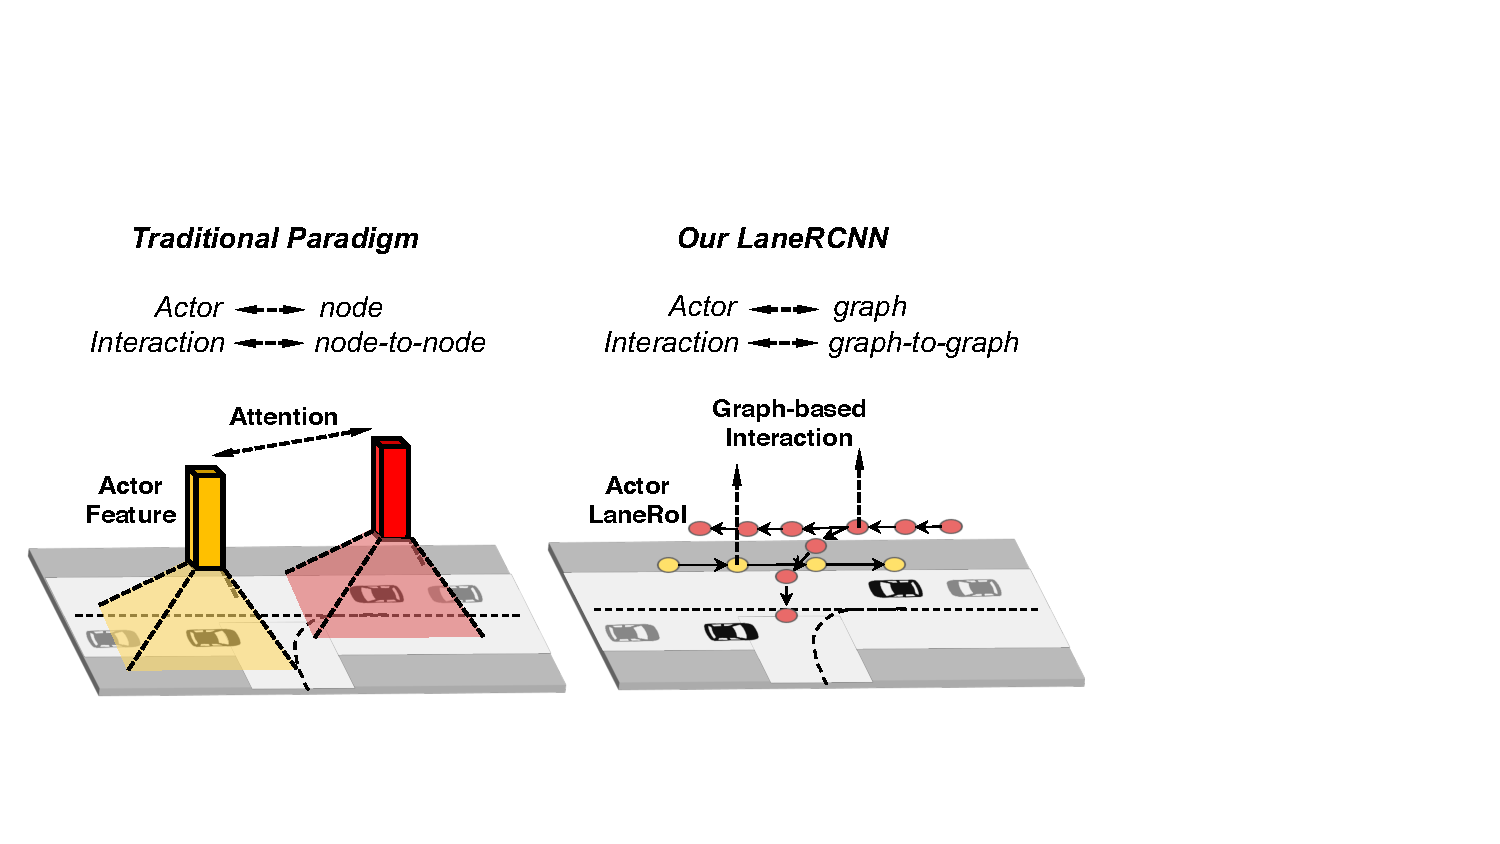
\includegraphics[height=3.4cm]{figures/teaser.pdf}
\end{center}
\vspace{-0.2cm}
\caption{Popular motion forecasting methods encode actor and its context
information into a feature vector, and treat it as a node in an interaction graph.
In contrast, we propose a graph-based
representation \ROI per actor, which is structured and expressive. Based on
it, we model interactions and forecast motion in a map topology aware manner.}
\vspace{-0.2cm}
\label{fig:teaser}
\vspace{-0.2cm}
\end{figure}



\begin{figure*}[t]
\begin{center}
  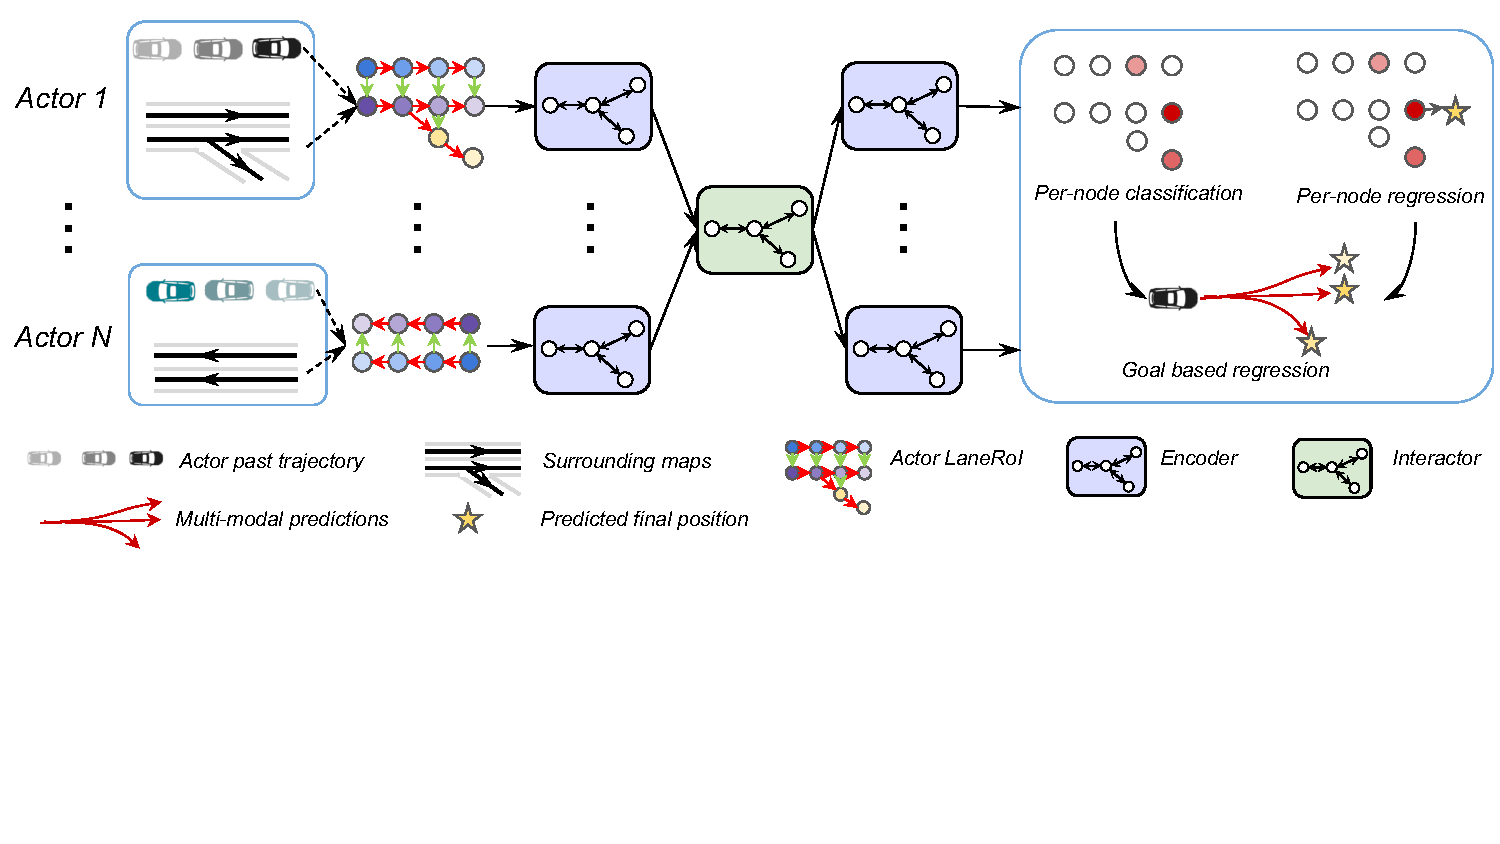
\includegraphics[height=6.0cm]{figures/lanercnn.pdf}
\end{center}
\vspace{-0.3cm}
\caption{Overview of LaneRCNN. It first
encodes each actor with our proposed \ROI representation, processes
each \ROI with an encoder, and then models interactions among actors with a
graph-based interactor. Finally, LaneRCNN predicts final positions of actors in
a fully-convolutional manner, and then decodes full trajectories based on these
positions.}
\vspace{-0.1cm}
\label{fig:lanercnn}
\end{figure*}

Although such a paradigm has shown competitive results, it has three main shortcomings:
1) Representing the context information of large regions of space, such as fast
moving actors traversing possibly a hundred meters within five seconds, with a
single vector is difficult, as we will show in our experiments.
2) Building a fully-connected interaction graph among actors ignores important map
structures~\cite{lgn,vectornet}. For example, an unprotected left turn vehicle should yield to oncoming traffic, while two
spatially nearby vehicles driving on opposite lanes barely interact with each other.
3) The regression header does not explicitly leverage the lane information, which could provide a good inductive bias for accurate predictions. 
As a consequence, regression-based
predictors sometimes forecast \textit{shooting-out-of-road} trajectories, which
are unrealistic. 






In this paper, we propose a graph-centric motion forecasting model, \ie, LaneRCNN, 
to address the aforementioned issues. 
We represent an actor and its context 
in a distributed and map-aware manner by 
constructing an actor-specific graph, called Lane-graph Region-of-Interest (\textit{LaneRoI}), along with node 
embeddings that encode the past motion and map semantics. 
In particular, we construct  \textit{LaneRoI} following the topology 
of lanes that are relevant to this actor, where nodes on this graph correspond
to small spatial regions along these lanes, and edges represent the topological and spatial relations among regions. 
Compared to using a single vector to encode all the information of a large region, our \textit{LaneRoI} naturally
preserves the map structure and captures the more fine-grained information, 
as each node embedding only needs to represent the local context within a small
region. 
To model interactions, we embed the \textit{LaneRoI}s of all actors to
a global lane graph  and then propagate the information over this global graph.
Since the \textit{LaneRoI}'s of interacting actors are highly relevant, those actors will
share overlapping regions on the global graph, thus having more frequent
communications during the information propagation compared to 
irrelevant actors. 
Importantly, this process neither requires any heuristics nor makes any oversimplified
assumptions while learning interactions conditioned on maps. 
We then predict future motions on each
\textit{LaneRoI} in a \emph{fully-convolutional} manner, such that small regions along
lanes (nodes in \textit{LaneRoI}) can serve as anchors and provide good priors
. We demonstrate the effectiveness of our method on the
large-scale Argoverse motion forecasting benchmark \cite{argoverse}, and
achieve state-of-the-art performance evaluated by the official ranking metric.




\section{Related Work}

\paragraph{Motion Forecasting:}
Traditional methods use hand-crafted features and rules based on human knowledge 
to model interactions and constraints in motion forecasting
\cite{choi2013understanding,choi2012unified,deo2018would,helbing1995social,mehran2009abnormal,yamaguchi2011you,weichiuplay}, which are sometimes oversimplified and not scalable. 
Recently, learning-based approaches employ the deep learning and
significantly outperform traditional ones.
Given the actors and the scene, a deep
forecasting model first needs to design a format to encode the information.
To do so, previous methods \cite{precog,chauffeurnet,covernet} often rasterize
the trajectories of
actors into a Birds-Eye-View (BEV) image, with different channels representing
different observation timesteps, and then apply a CNN and RoI pooling
\cite{fasterrcnn,maskrcnn} to extract actor features. 
Maps can be encoded similarly
\cite{nmp,dsd,intentnet,chauffeurnet,mfp}. 
However, the square receptive fields of a CNN may not be efficient to
encode actor movements \cite{lgn}, which are typically long curves.
Moreover, the map rasterization may lose useful information like lane topologies. 
RNNs are an alternative way to encode actor kinematic information
\cite{matf,mfp,vectornet,tnt,socialgan,sociallstm} compactly and efficiently.
Recently, VectorNet \cite{vectornet} and LaneGCN \cite{lgn} generalized such compact encodings to map representations. 
VectorNet treats a map
as a collection of polylines and uses a RNN to encode them, while LaneGCN builds a
graph of lanes and conducts convolutions over the graph. Different from all these
work, we encode both actors and maps in an unified graph representation, which
is more structured and powerful.


Modeling interactions among actors is also critical for
a multi-agent system. Pioneering learning-based work design a social-pooling mechanism
\cite{sociallstm,socialgan} to aggregate the information from nearby actors.
However, such a 
pooling operation may potentially lose
actor-specific information. To address this,
attention-mechanism \cite{sophie,socialatt,carnet,sun2019relational} or GNN-based
methods \cite{dsd,interacttransformer,lgn,spagnn,precog,mfp,ilvm,vectornet} build actor
interaction graphs (usually fully-connected with all actors or k-nearest
neighbors based),
and perform attention or message passing to update actor features.
Social convolutional pooling \cite{matf,socialconvpool,pip} has also been explored, which maintains the spatial
distribution of actors. 
However, most of these work do not explicitly consider map structures,
which largely affects interactions among actors in reality. 

To generate each actor's predicted futures, many works sample multi-modal futures under a conditional variational auto-encoder (CVAE) framework
\cite{desire,r2p2,mfp,precog,ilvm}, or with a multi-head/mode regressor
\cite{lgn,cui2019multimodal,mercat2020multi}.
Others output discrete sets of
trajectory samples \cite{dsd,covernet,multipath} or occupancy maps
\cite{jain2019discrete,p3}. Recently, TNT \cite{tnt}
concurrently and independently designs a similar output parameterization as ours
where lanes are used as priors for the forecasting. 
Note that, in addition to the parameterization, we contribute a novel graph representation and a powerful
architecture which significantly outperforms their results.



\paragraph{Graph Neural Networks:}


Relying on operators like graph convolution and message passing, graph neural networks (GNNs) and their variants \cite{scarselli2008graph,bruna2013spectral,li2015gated,kipf2016semi,hamilton2017inductive,liao2019lanczosnet} generalize deep learning on regular graphs like grids to ones with irregular topologies.
They have achieved great successes in learning useful graph representations for
various tasks \cite{monti2017geometric,qi20173d,teney2017graph,li2017situation,garcia2018few}.
We draw inspiration from the general concept ``ego-graph'' and propose \textit{LaneRoI}, which is specially designed for lane graphs and captures both the local map topologies and the past motion information of an individual actor.
Moreover, to capture interactions among actors, we further propose an
interaction module which effectively communicates information among
\textit{LaneRoI} graphs.



\section{LaneRCNN}


Our goal is to  predict the future motions of all actors in a scene, given their
past motions and an HD map. Different from existing work, we represent an actor
and its context with a \textit{LaneRoI}, an actor-specific graph representation which is more
structured and expressive than the single feature vector used in the literature. 
Based
on this representation, we design LaneRCNN, a graph-centric motion forecasting
model that encodes context, models interactions between actors, and predicts future motions all in
a map topology aware manner. An overview of our model is shown in
Fig.~\ref{fig:lanercnn}.

In the following, we first introduce our problem formulation 
in Sec. \ref{sec:notation}. We then define our \ROI representations in Sec.
\ref{sec:laneroi}. In Sec. \ref{sec:backbone}, we explain how LaneRCNN processes features and models interactions via graph-based message-passing. 
Finally, we show our map-aware trajectory decoder and learning
in Sec. \ref{sec:output} and Sec. \ref{sec:learning} respectively.






\subsection{Problem Formulation}
\label{sec:notation}
We denote the  past motion of the $i$-th actor as a set of 2D points encoding
the center locations over the past $L$ 
 timesteps, \ie, $\left\{(x_i^{-L}, y_i^{-L}), \cdots, (x_i^{-1},
y_i^{-1})\right\}$, with $(x,y)$  the  2D coordinates  in bird's eye view (BEV). Our goal is to forecast the future motions of all actors in the scene 
$\left\{(x_i^{1}, y_i^{1}), \cdots, (x_i^{T}, y_i^{T}) | i = 1, \cdots, N\right\}$,
where $T$ is our prediction horizon and $N$ is the number of actors. 

In addition to the past kinematic information of the actors, maps also play an important role 
for motion forecasting since (i) actors usually follow lanes on the map, 
(ii) the map structure determines the right of way, which in turns affects the interactions among actors.
As is common practice in self-driving, we assume an HD map is accessible, 
which contains lanes and associated semantic attributes, \eg,
traffic light information. 
Each lane is composed of
many consecutive lane segments $\ell_i$, which are short segments
along the centerline of the lane.
In addition, a lane segment $\ell_i$ can have pairwise relationships with
another segment $\ell_j$ in the same or another lane, 
such as $\ell_i$ being a successor of $\ell_j$ or a left neighbor.

\subsection{LaneRoI Representation}
\label{sec:laneroi}


\paragraph{Graph Representation}
One straight-forward way to represent an actor and its context (map) information
is by first rasterizing both its trajectory as well as the map to form a 2D BEV
image, and then apply cropping centered in the actor's location in BEV \cite{dsd, mfp, matf, spagnn}.
However, rasterizations are prone to information loss such as 
connectivities among lanes. 
Furthermore, it is a rather inefficient representation
since actor motions are expanded typically in the direction along the lanes, not across them. 
Inspired by \cite{lgn}, we instead use a graph representation for our \ROI to
preserve the structure while being compact. For each actor $i$ in the scene, we first
retrieve all relevant lanes that this actor can possibly go to in the prediction horizon
$T$ as well as come from in the observed history horizon $L$. We then convert the
lanes into a directed graph $\G_i =
\{\mathcal{V}, \{ \mathcal{E}_\text{suc}, \mathcal{E}_\text{pre},
    \mathcal{E}_\text{left}, \mathcal{E}_\text{right} \}\}$
where each node $v \in \mathcal{V}$ represents a lane segment within those lanes 
and the lane topology is represented by different types of edges $\mathcal{E}_r$,
encoding the following relationships: predecessor, successor, left
and right neighbor.  
Two nodes are connected by an edge $e \in \mathcal{E}_r$ if the corresponding lane segments $\ell_i,
\ell_j$ have a relation $r$, \eg, lane segment $\ell_i$ is a
successor of lane segment $\ell_j$.
Hereafter, we will use the term node interchangeably with the term lane segment. 











\paragraph{Graph Input Encoding}
The graph $\G_i$ only characterizes map structures around the $i$-th actor without much information about the actor.
We therefore augment the graph with a set of node embeddings to
construct our \textit{LaneRoI}.
Recall that each node $k$ in $\G_i$ is associated with a lane
segment $\ell_k$. We design its embedding $f_k \in \mathbb{R}^C$ 
to capture the geometric and semantic information of
$\ell_k$, as well as its relations with the actor, where $C$ denotes the feature
dimension.
In particular, geometric features include the center location, the orientation and the
curvature of $\ell_k$; semantic features include binary features indicating if
$\ell_k$ is a turning lane,  if it is currently controlled by a red light,
\etc. To encode the actor information into $f_k$, we note that the past motion of an
actor can be identified as a set of 2D displacements, defining the 
movements between consecutive timesteps. Therefore, we also include the relative
positions and orientations of these 2D displacements \wrt $\ell_k$
into $f_k$ which encodes actor motions in a map-dependent manner.
This is beneficial for understanding actor behaviors \wrt the map, \eg, a trajectory that 
steadily deviates from one lane and approaches the neighboring lane is highly likely 
a lane change.
In practice, it is important to clamp the actor information, \ie, if $\ell_k$ is more than 5 meters away from the
actor we replace the actor motion embedding in $f_k$ with zeros. 
We hypothesize that such a restriction encourages the model to learn better representations via the message passing over the graph.
To summarize, $(\G_i, \mathbf{F}_i)$ is the \ROI of the actor $i$, encoding
the actor-specific information for motion forecasting,
where $\mathbf{F}_i \in
\mathbb{R}^{M_i \times C}$ is the collection of node embeddings $f_k$ and 
$M_i$ is the number of nodes in $\G_i$. 

\begin{figure}[t]
\begin{center}
  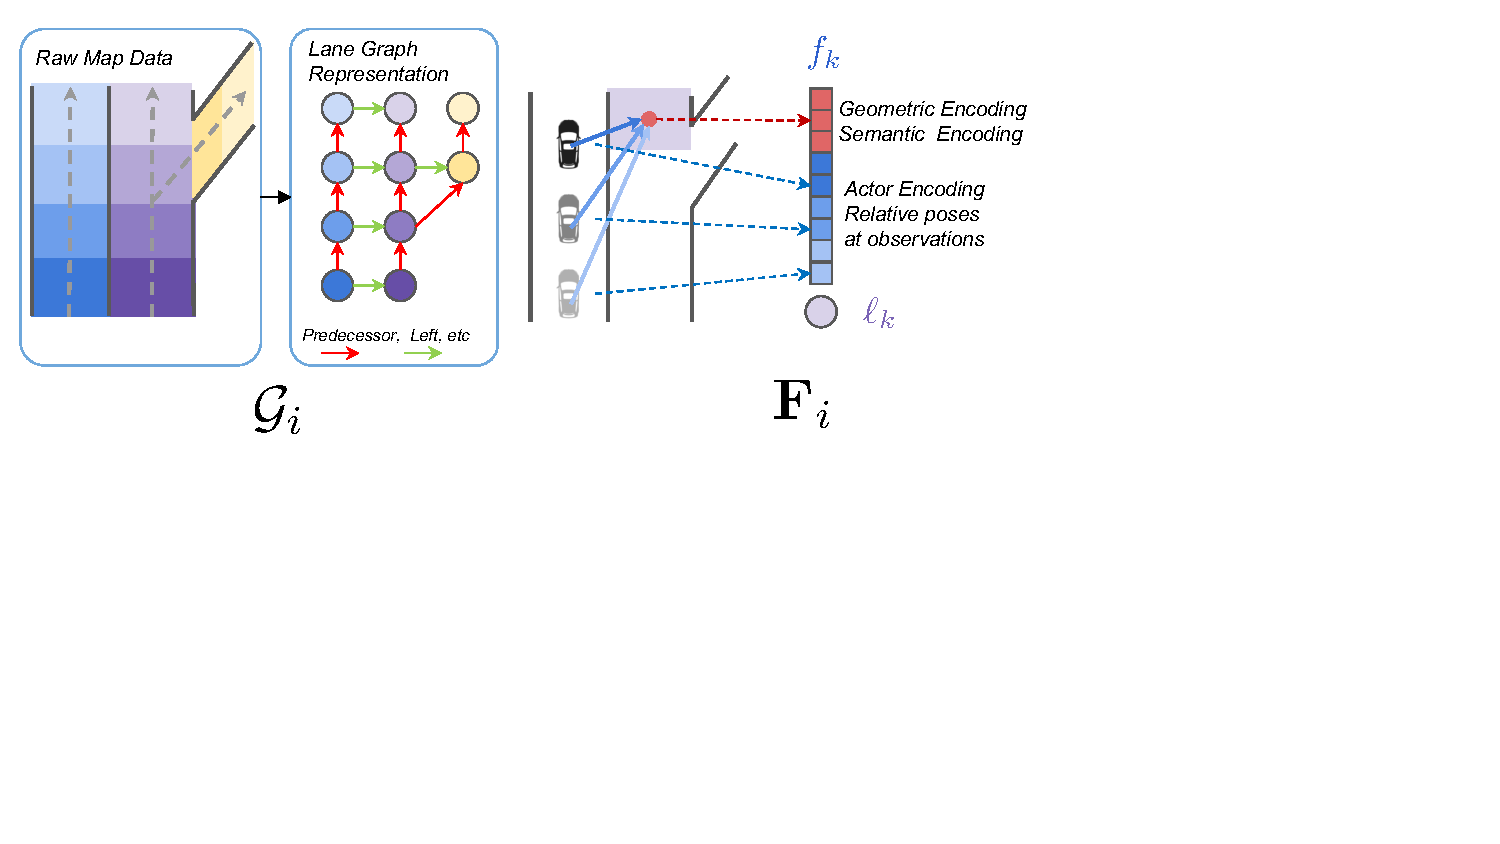
\includegraphics[height=3.4cm]{figures/laneroi.pdf}
\end{center}
\vspace{-0.2cm}
\caption{
The LaneRoI of the actor $i$ is a collection of a graph $\G_i$ (constructed following lane topology: nodes as
lane segments and edges as segment connectivities) and node
embeddings $\mathbf{F}_i$ (encoding motions of the actor, as well as
geometric and semantic properties of lane segments).}
\vspace{-0.3cm}
\label{fig:laneroi}
\end{figure}


\subsection{LaneRCNN Backbone}
\label{sec:backbone}
As \textit{LaneRoI}s have irregular graph structures, we can not apply standard
2D convolutions to obtain feature representations. In the following, we first introduce
the lane convolution and pooling operators (Fig.~\ref{fig:operator}), which serve similar
purposes as their 2D counterparts while respecting the graph topology. 
Based on these operators, we then describe how our LaneRCNN updates features of
each \ROI as well as handles interactions among all \textit{LaneRoI}s (actors).


\paragraph{Lane Convolution Operator}
We briefly introduce the lane convolution which was originally proposed in \cite{lgn}
Given a \ROI $(\G_i, \mathbf{F}_i)$, 
a lane convolution updates features $\mathbf{F}_i$ by aggregating features from
its neighborhood (in the graph). 
Formally, we use $\E_i(r)$ to denote the 
binary adjacency matrix for $\G_i$ under the relation $r$, \ie, the $(p, q)$ entry 
in this matrix is $1$ if lane segments $\ell_p$ and $\ell_q$ have the relation $r$ 
and $0$ otherwise. 
We denote the $n$-hop connectivity under the relation $r$ as the matrix 
$\bool\left(\E_i(r) \cdot \E_i(r) \cdots \E_i(r)\right) = \bool
\left(\E_i^n(r)\right)$, where the operator $\bool$ sets any non-zero entries to one 
and otherwise keeps them as zero. 
The output node features are updated as follows,
\begin{equation}
  \label{eq:conv}
  \mathbf{F}_i \leftarrow \Psi \left( \mathbf{F}_i\mathbf{W} + \sum_{r, n}
  \bool \left(\E_i^n(r)\right)\mathbf{F}_i\mathbf{W}_{n, r} \right),
\end{equation}
where both $\mathbf{W}$ and $\mathbf{W}_{n, r}$ are learnable
parameters, $\Psi(\cdot)$ is a non-linearity consisted of
LayerNorm \cite{layernorm} and ReLU \cite{relu},
and the summation is over all possible relations $r$
and hops $n$. In practice, we use 
$n \in \left\{1, 2, 4,
8, 16, 32\right\}$.
Such a multi-hop mechanism mimics the dilated convolution \cite{yu2015multi} and effectively enlarges
the receptive field.

\begin{figure}[t]
\begin{center}
  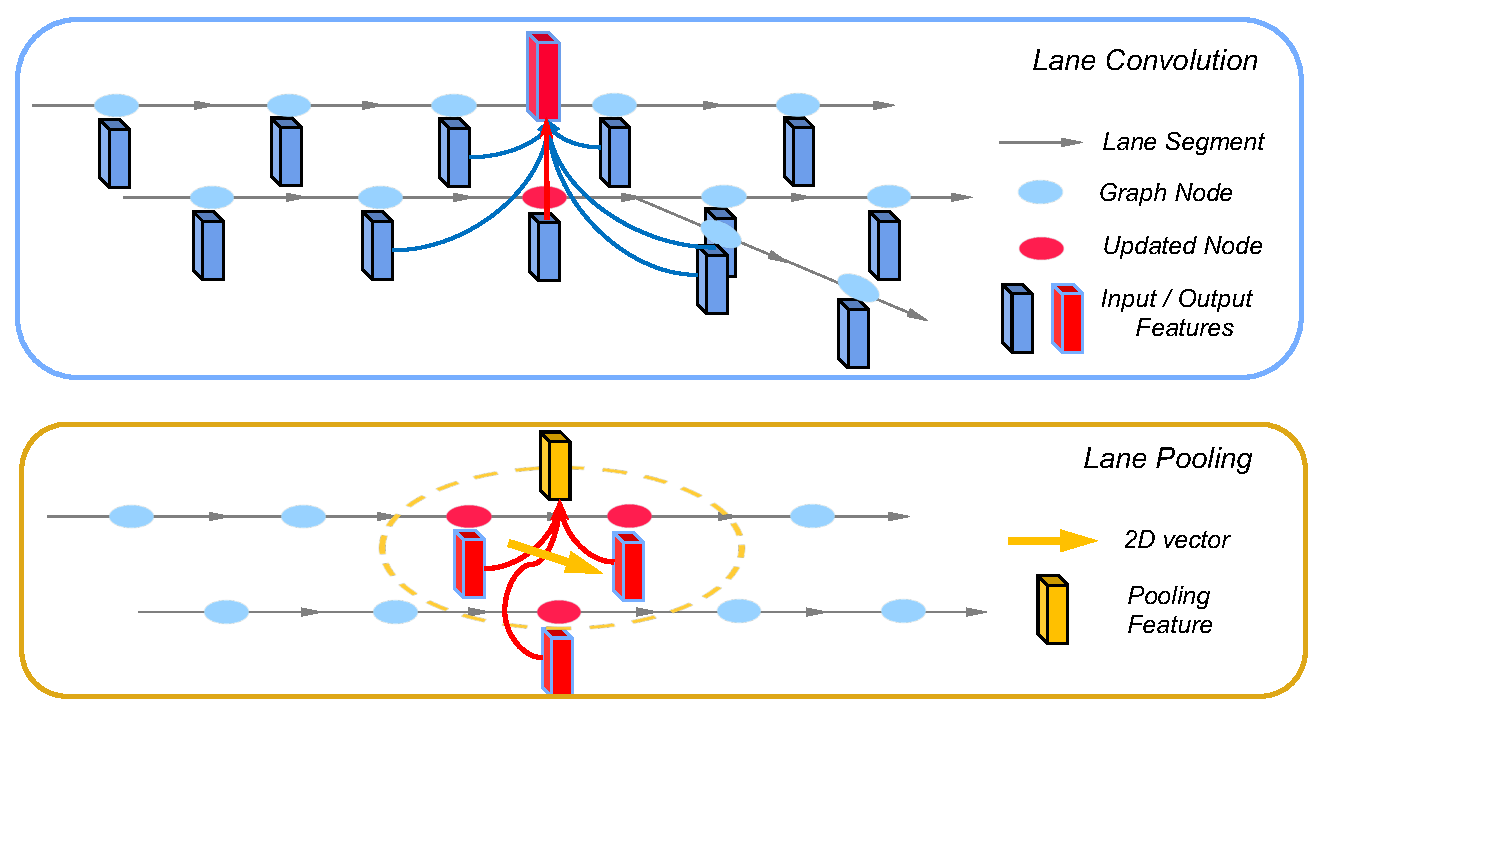
\includegraphics[height=4.5cm]{figures/operator.pdf}
\end{center}
\vspace{-0.2cm}
\caption{An illustration for lane convolution and lane
pooling operators, which have similar functionalities as their 2D counterparts
while respecting the lane topology.}
\label{fig:operator}
\end{figure}


\paragraph{Lane Pooling Operator}
We use a learnable pooling function for lane pooling operator.
Given a \ROI
$(\G_i, \mathbf{F}_i)$, recall $\G_i$ actually corresponds to a number of
lanes spanned in the 2D plane (scene). For an arbitrary 2D vector
$\mathbf{v}$ in the plane, a lane pooling operator pools, or `interpolates',
the feature of $\mathbf{v}$ from $\mathbf{F}_i$. Note that
$\mathbf{v}$ can be a lane segment in another graph $\G_j$ (spatially
close to $\G_i$). Therefore, lane pooling helps
communicate information back and forth between graphs, which we will explain in the interaction part.
To generate the feature $f_\mathbf{v}$ of vector $\mathbf{v}$, we first retrieve
its `neighboring nodes' in $\G_i$, by checking if the center distance between a lane segment
$\ell_k$ in $\G_i$ and vector $\mathbf{v}$ is smaller than a certain threshold. A naive
pooling strategy is to simply take a mean of those $\ell_k$. However, this
ignores the fact that relations between $\ell_k$ and $\mathbf{v}$ can vary a lot
depending on their relative pose: a lane segment that is perpendicular to
$\mathbf{v}$ (conflicting) and the one that is aligned with $\mathbf{v}$
have very different semantics. Inspired by the generalized convolution on graphs/manifolds
\cite{monti2017geometric, contconv, lgn}, we use the relative pose and some non-linearities to
learn a pooling function. In particular, we denote the set of surrounding
nodes on $\G_i$ as $\mathcal{N}$, and the relative pose between $\mathbf{v}$ and
$\ell_k$ as $\Delta_{\mathbf{v}k}$ which includes relative position and
orientation. The pooled feature $f_{\mathbf{v}}$ can then be written as,
\begin{equation}
  \label{eq:pool}
  f_{\mathbf{v}} = \mathcal{M}_b\left(\sum_{k\in \mathcal{N}}
    \mathcal{M}_a\left(\left[
        f_k, \Delta_{\mathbf{v}k}
\right]\right)\right),
\end{equation}
where $[\cdots]$ means concatenation and $\mathcal{M}$
is a two-layer multi-layer perceptron (MLP).



\begin{table*}[t]
\vspace{-0.2cm}
\centering
\begin{tabular}{l|>{\columncolor{grey}}cccccc}
  \specialrule{.2em}{.1em}{.1em}
  Method & MR (K=6) & minADE (K=6) & minFDE (K=6) & MR (K=1) & minADE (K=1) & minFDE (K=1) \\
  \hline
   NN+Map~\cite{argoverse} & 58.0 & 2.08 & 4.02 & 94.0 & 3.65 & 8.12\\
   LSTM+Map~\cite{argoverse} & 67.0 & 2.08 & 4.19 & 75.0 & 2.92 & 6.45\\
   UULM-MRM~\cite{argoleaderboard} & 21.8 & 0.97 & 1.55 & 63.4 & 1.90 & 4.19\\
   WIMP~\cite{wimp} & 16.7 & 0.99 & 1.67 & 62.9 & 1.82 & 4.03\\ 
   VectorNet~\cite{vectornet} & - & - & - & - & 1.81 & 4.01\\
   LaneGCN~\cite{lgn} & 16.3 & \textbf{0.87} & \textbf{1.36} & 59.0 & 1.71 & 3.78\\
   SAMMP~\cite{mercat2020multi} & 13.3 & 0.94 & 1.54 & 59.7 & 1.78 & 3.91\\
   TNT~\cite{tnt} & 13.3 & 0.94 & 1.54 & 59.7 & 1.78 & 3.91\\
   % NN+map & 3.65 & 8.12 & 94.0 & 2.08 & 4.02 & 58.0 \\
   % LSTM+map & 2.92 & 6.45 & 75.0 & 2.08 & 4.19 & 67.0 \\
   % TNT (4th) \cite{tnt} & 1.78 & 3.91 & 59.7 & 0.94 & 1.54 & 13.3   \\
   % Jean (3rd) \cite{mercat2020multi} & 1.74 & 4.24 & 68.6 & 1.00 & \textbf{1.42} & 13.1  \\
   % Poly (2nd) \cite{argoleaderboard} & 1.71 & 3.85 & 59.6 & \textbf{0.89} & 1.50 & 13.1 \\
   \hline
   Ours-LaneRCNN & \textbf{12.3} & 0.90 & 1.45 & \textbf{56.9}
                       &\textbf{1.69} &\textbf{3.69}\\
   % \textbf{1.69} & \textbf{3.69} & \textbf{56.9} & 0.90 & 1.45 & \textbf{12.3} \\
  \specialrule{.1em}{.05em}{.05em}


\end{tabular}
\caption{Argoverse Motion Forecasting Benchmark (test set). All metrics are lower the
  better and \colorbox{grey}{Miss-Rate (MR, K=6)} is the official ranking metric.}
\label{table:argo}
\vspace{-0.2cm}
\end{table*}





\paragraph{LaneRoI Encoder}
Equipped with operators introduced above, we now describe how LaneRCNN processes
features for each \textit{LaneRoI}. Given a scene, we first
construct a \ROI per actor and encode its input information into node
embeddings as described in Sec. \ref{sec:laneroi}. Then, for each \textit{LaneRoI}, we apply
four lane convolution layers and get the updated node embeddings
$\mathbf{F}_i$.
Essentially, a lane convolution layer propagates information from a node to
its (multi-hop) connected nodes. Stacking more layers builds larger receptive
fields and has a larger model capacity. However, we find deeper
networks do not necessarily lead to better performances in practice, possibly due to the well-known
difficulty of learning long-term dependencies. To address this, we introduce a
graph shortcut mechanism on \textit{LaneRoI}. 
The graph shortcut layer can be applied after any layer of lane convolution:
we aggregate $\mathbf{F}_i$ output from the previous layer into a global
embedding with the same dimension as node embeddings, and then add it to embeddings
of all nodes in $\G_i$.
Recall that the actor past motions are a number of 2D vectors, \ie, movements
between consecutive timesteps. We use the lane pooling to extract
features for these 2D vectors. A 1D CNN with downsampling is then applied to these features to
build the final shortcut embedding. Intuitively, a lane convolution may suffer
from the diminishing information flow during the message-passing, while such
a shortcut can provide an auxiliary and shorter path to communicate among far-away nodes
efficiently. We will show that the shortcut significantly boosts the performance in the ablation study.



\paragraph{LaneRoI Interactor}
So far, our \ROI encoder provides good features for a given actor, but it
lacks the ability to model interactions among different actors, which is
extremely important for the motion forecasting in a multi-agent system. We now
describe  how we handle actor interactions under \ROI representations.
After processing all \textit{LaneRoI}s with the \ROI encoder (shared weights), we build a global lane graph
$\G$ containing all lanes in the scene. Its node embeddings are constructed by
projecting all \textit{LaneRoI}s to $\G$ itself. We then apply four lane convolution layers on $\G$ to perform message passing. Finally, we distribute the
`global node' embeddings back to each \textit{LaneRoI}. Our design is motivated by the fact
that \textit{actors have interactions since they share the same space-time region}. 
Similarly, in our model, all \textit{LaneRoI}s share the same global graph $\G$ and
communicate with each other following $\G$.

In particular, suppose we have a set of \textit{LaneRoI}s $\{(\G_i,
\mathbf{F}_i)|i=1,\cdots,N\}$ encoded from previous layers and a global lane
graph $\G$. For each node in $\G$, we use a lane pooling to construct its
embedding: retrieving its neighbors from all \textit{LaneRoI}s as $\mathcal{N}$,
measured by center distance, and then applying Eq. \ref{eq:pool}. This ensures
each global node has the information of all those actors that could 
interact with it. The distribute step is an inverse process: for each node in
$\G_i$, find its neighbors, apply a lane pooling, and add the resulted embedding to original $\mathbf{F}_i$ (serving as a
skip-connection).

% \begin{table*}[t]
% \vspace{-0.2cm}
% \centering
% \begin{tabular}{l|l|ccc|cc>{\columncolor{grey}}c}
%   \specialrule{.2em}{.1em}{.1em}
%  & \multirow{2}{*}{Method} & \multicolumn{3}{c|}{K=1} & \multicolumn{3}{c}{K=6} \\
%  & & minADE & minFDE & MR & minADE & minFDE & MR \\
%   \hline
%   \multirow{3}{*}{Argoverse Baseline \cite{argoverse}} & NN & 3.45 & 7.88 & 87.0 & 1.71 & 3.28& 53.7 \\
%                        & NN+map & 3.65 & 8.12 & 94.0 & 2.08 & 4.02 & 58.0 \\
%                        & LSTM+map & 2.92 & 6.45 & 75.0 & 2.08 & 4.19 & 67.0 \\
%   \hline
%   \multirow{4}{*}{Leaderboard \cite{argoleaderboard}} & TNT (4th) \cite{tnt} & 1.78 & 3.91 & 59.7 & 0.94 & 1.54 & 13.3   \\
%                                & Jean (3rd) \cite{mercat2020multi} & 1.74 & 4.24 & 68.6 & 1.00 & \textbf{1.42} & 13.1  \\
%                                & Poly (2nd) \cite{argoleaderboard} & 1.71 & 3.85 & 59.6 & \textbf{0.89} & 1.50 & 13.1 \\
%                                \cline{2-8}
%                    & Ours-LaneRCNN (1st) & \textbf{1.69} & \textbf{3.69} &
%   \textbf{56.9} & 0.90 & 1.45 &
%   \textbf{12.3} \\
%   \specialrule{.1em}{.05em}{.05em}


% \end{tabular}
% \caption{Argoverse Motion Forecasting Leaderboard. All metrics are lower the
%   better and \colorbox{grey}{Miss-Rate (MR, K=6)} is the official ranking metric.}
% \label{table:argo}
% \vspace{-0.2cm}
% \end{table*}



\subsection{Map-Relative Outputs Decoding}
\label{sec:output}

The future is innately multi-modal and an actor can take many different yet possible
future motions. Fortunately, different modalities can be largely characterized by
different goals of an actor. Here, a goal means a
final position of an actor at the end of prediction horizon. Note that actors
mostly follow lane structures and thus their goals are usually close to a lane
segment $\ell$. Therefore, our model can predict the final goals of an actor in a
fully convolutional manner, based on its \ROI features. Namely, we apply a
2-layer MLP on each node feature $f_k$, and output five values including the
probability that $\ell_k$ is the closest lane segment to destination 
$p(\ell_k=\text{goal})$, as well as relative residues from $\ell_k$ to the final
destination $x_{gt} - x_{k}$, $y_{gt} - y_{k}$, $\sin(\theta_{gt} - \theta_k)$,
$\cos(\theta_{gt} - \theta_k)$.

Based on results of previous steps, we select the top K\footnote{On
Argoverse, we follow the official metric and use K=6.} predictions.
% We also remove duplicate
% goals if two predictions are too close, where the lower confidence one is
% ignored.} 
For each predicted goal, we use the position and the direction of the actor at
$t=0$ as well as those at the goal to interpolate a Bezier quadratic curve.
We then sample 2D points at each future timestep by unrolling a constant 
acceleration kinematic model along this curve.
These 2D points form a trajectory, which serves as an initial proposal of our final forecasting.
Despite its simplicity, this parameterization gives us surprisingly good results.

Our final step is to refine those trajectory proposals using a learnable header. 
Similar to the shortcut layer introduced in Sec.
\ref{sec:backbone}, we use a lane pooling followed by a 1D CNN to 
pool features of this trajectory. 
Finally, we decode a pair of values per timestep, representing the residue from the trajectory proposal to the
ground-truth future position at this timestep (encoded in Frenet coordinate of
this trajectory proposal). 
% We provide more detailed definitions of our parameterization and output space in the supplementary~\ref{sec:supp_output}.



\subsection{Learning}
\label{sec:learning}
We train our model end-to-end with a loss containing the goal classification, the goal
regression, and the trajectory refinements. Specifically, we use
$$
\label{eq:objective}
\mathcal{L} = \mathcal{L}_{\text{cls}} + \alpha\mathcal{L}_{\text{reg}} +
\beta\mathcal{L}_{\text{refine}},
$$
where $\alpha$ and $\beta$ are hyparameters.
As our model predicts the goal classification and regression results per node, we simply adopt a binary cross entropy loss for $\mathcal{L}_{\text{cls}}$ with online hard example mining \cite{ohem} and a smooth-L1 loss for $\mathcal{L}_{\text{reg}}$, where
the $\mathcal{L}_{\text{reg}}$ is only evaluated on positive nodes, \ie closest lane
segments to the ground-truth final positions. The $\mathcal{L}_{\text{refine}}$ is also
a smooth-L1 loss with training labels generated on the fly: projecting
ground-truth future trajectories to the predicted trajectory proposals, and use
the Frenet coordinate values as our regression targets.






























\begin{table*}[t]
\centering
\begin{tabular}{c|cc|cc|ccc}
  \specialrule{.2em}{.1em}{.1em}
  \multirow{2}{*}{Module} & \multicolumn{2}{c|}{\multirow{2}{*}{Ablation}} &
  \multicolumn{2}{c|}{K=1} & \multicolumn{3}{c}{K=6} \\
 & & & minADE & minFDE & minADE & minFDE & MR \\
  \hline
  \multirow{7}{*}{LaneRoI Encoder} & \ROI & Shortcut & & & & & \\
  \cline{2-8}
              & & & 1.68 & 3.79 & 0.86 & 1.46 & 14.5 \\
  & \checkmark & & 1.68 & 3.84 & 0.82 & 1.36 & 12.9 \\
  & \checkmark & Global Pool & 1.69 & 3.84 & 0.84 & 1.38 & 12.8 \\
  & \checkmark & Center Pool & 1.67 & 3.80 & 0.83 & 1.35 & 12.4 \\
  & \checkmark & Ours x 1 & 1.55 & 3.45 & 0.81 & \textbf{1.29} & 11.1 \\
  \rowcolor{grey} \cellcolor{white}& \checkmark & Ours x 2 & \textbf{1.54} &
  \textbf{3.45} & \textbf{0.80} & \textbf{1.29} & \textbf{10.8}\\
  \specialrule{.1em}{.05em}{.05em}
  \specialrule{.1em}{.05em}{.05em}
  \multirow{8}{*}{LaneRoI Interactor} & Interactor-Arch & Pooling & & & & & \\
  \cline{2-8}
                              & & & 1.54 & 3.45 & 0.80 & 1.29 & 10.8 \\
  & Attention & Global & 1.42 & 3.10 & 0.78 & 1.24 & 9.8 \\
  & Attention & Shortcut & 1.47 & 3.22 & 0.80 & 1.25 & 10.1 \\
  & GNN & Global & 1.45 & 3.15 & 0.79 & 1.25 & 9.9 \\
  & GNN & Shortcut & 1.45 & 3.21 & 0.79 & 1.25 & 10.0 \\
  & Ours & AvgPool & 1.42 & 3.11 & 0.79 & 1.25 & 9.9 \\
  \rowcolor{grey} \cellcolor{white} & Ours & LanePool & \textbf{1.33} &
  \textbf{2.85} & \textbf{0.77} & \textbf{1.19} & \textbf{8.2}\\
  \specialrule{.1em}{.05em}{.05em}

\end{tabular}
\caption{Ablations on different modules of LaneRCNN. Metrics are reported on the validation set.
In the upper half, we examine our \ROI Encoder, comparing per-actor 1D feature vector 
v.s. \ROI representations as well as different designs for the shortcut mechanism.
In the lower half, we compare different strategies to model interactions, including a
fully connected graph among actors with GNN / attention, as well as ours.
Pooling refers to how we pool a 1D actor feature from each \ROI which are
used by GNN / attention. Rows in gray indicate the architecture used in
our final model.}
\label{table:ablation}
\end{table*}




\section{Experiment}

We evaluate the effectiveness of LaneRCNN on the large-scale Argoverse motion
forecasting benchmark (Argoverse), which is publicly available and provides annotations
of both actor motions and HD maps. In the following, we first
explain our experimental setup and then compare our method against
state-of-the-arts. We also conduct ablation studies on each
module of LaneRCNN to validate our design choices. Finally, we present some
qualitative results.

\subsection{Experimental Settings}
\paragraph{Dataset}
Argoverse provides a large-scale dataset \cite{argoverse} for the
motion forecasting task, which is to
forecast 3 seconds future motions of a particular actor (labeled with type
`agent') given 2 seconds past observations of all
actors in the scene, sampled at 10Hz. 
This dataset consists of more than 30K real-world driving sequences collected in Miami and Pittsburgh.
Those sequences are further split into train, validation, and test sets without
any geographical overlapping. 
% Each of them has 205942, 39472, and 78143 sequences
% respectively. In particular, each sequence contains the positions of all actors in
% a scene within the past 2 seconds history, annotated at 10Hz.
% For each sequence, it specifies one interesting actor in this scene, with type `agent', whose future 3 seconds
% motions are used for the evaluation. 
% The train and validation splits additionally
% provide future locations of all actors within 3 second horizon labeled at 10Hz, while 
Annotations of future timesteps for test sequences are withheld from the public and used for
the leaderboard evaluation. Besides, HD map information can be retrieved for all
sequences. 

\paragraph{Metrics} We follow the benchmark setting and use Miss-Rate (MR), Average
Displacement Error (ADE) and Final Displacement Error (FDE), which are also
widely used in the community. MR is defined as the ratio of data that none of
the predictions has less than 2.0 meters L2 error at the final timestep. ADE is
the averaged L2 errors of all future timesteps, while FDE only
counts the final timestep. To evaluate the mutli-modal prediction, we
also adopt the benchmark setting: predicting K=6 future trajectories
per actor and evaluating the $\text{min}_{K}\text{MR}$, $\text{min}_{K}\text{ADE}$,
$\text{min}_{K}\text{FDE}$ using the trajectory that is closest to the
ground-truth.

\paragraph{Implementation Details}
We train our model on the \emph{train} set with the batch size of 64 and terminate at 30
epochs. We use Adam \cite{adam} optimizer with the learning rate initialized at 0.01 and decayed by 10 at 20 epochs. To normalize the data, we translate and rotate the coordinate system of each sequence so that
the origin is at current position ($t=0$) of `agent' actor and x-axis is aligned
with its current direction. During training, we further apply a random rotation
data augmentation within $(-\frac{2}{3}\pi, \frac{2}{3}\pi)$. No other data
processing is applied such as label smoothing. 
% More implementation details are provided in the supplementary~\ref{sec:supp_implement}.

\subsection{Comparison with State-of-the-art}
We compare our approach to several recent state-of-the-art methods and summarize
their performance on the test set in Table~\ref{table:argo}. Those methods
include: UULM-MRM~\cite{argoleaderboard} (rasterization based model, joint winner
of Argoverse Forecasting Challenge), WIMP~\cite{wimp} (recurrent graph-based
attention model), VectorNet~\cite{vectornet} (lane topology based GNN model),
LaneGCN~\cite{lgn} (lane topology based GCN model),
SAMMP~\cite{mercat2020multi} (self-attention based model, joint winner of
Argoverse Forecasting Challenge) and TNT~\cite{tnt} (target based model built
upon vectornet). Note that all of them largely beat the Argoverse baselines
(NN+Map and LSTM+Map), indicating this is a highly competitive benchmark.
Nevertheless, our method significantly outperform all previous method on the
official ranking metric (MR, K=6), and also beat most of the methods on other
metrics. 
% We compare our approach with top entries on Argoverse motion forecasting
% leaderboard \cite{argoleaderboard} as well as official baselines provided
% by the dataset \cite{argoverse} as shown in Table \ref{table:argo}. 
% We only submit our final model once to the leaderboard and achieve
% state-of-the-art performance.\footnote{Snapshot of the leaderboard at the submission time: Nov. 12, 2020.}
% This is a very challenging benchmark
% with around 100 participants at the time of our submission. Note that for the
% official ranking metric MR (K=6), previous leading methods are extremely close to
% each other, implying the difficulty of further improving the performance.
% Nevertheless, we significantly boost the number which verifies the
% effectiveness of our method. Among the competitors, both Jean
% \cite{mercat2020multi} and TNT \cite{tnt} use RNNs to encode actor kinematic
% states and lane polylines. They then build a fully-connected interaction graph
% among all actors and lanes, and use either the attention or GNNs to model
% interactions. As a result, they represent each actor with a single
% feature vector, which is less expressive than our \ROI representations. Moreover,
% the fully-connected interaction graph may also discard valuable map structure
% information. Note that TNT shares a similar output parameterization as
% ours, yet we perform better on all metrics. This further validates the advantages of
% our \ROI compared against traditional representations. Unfortunately, since Poly team does
% not publish their method, we can not compare with it qualitatively.


\begin{figure*}[t]
\vspace{-0.2cm}
\centering
\setlength{\tabcolsep}{1pt}
\begin{tabular}{cccc}
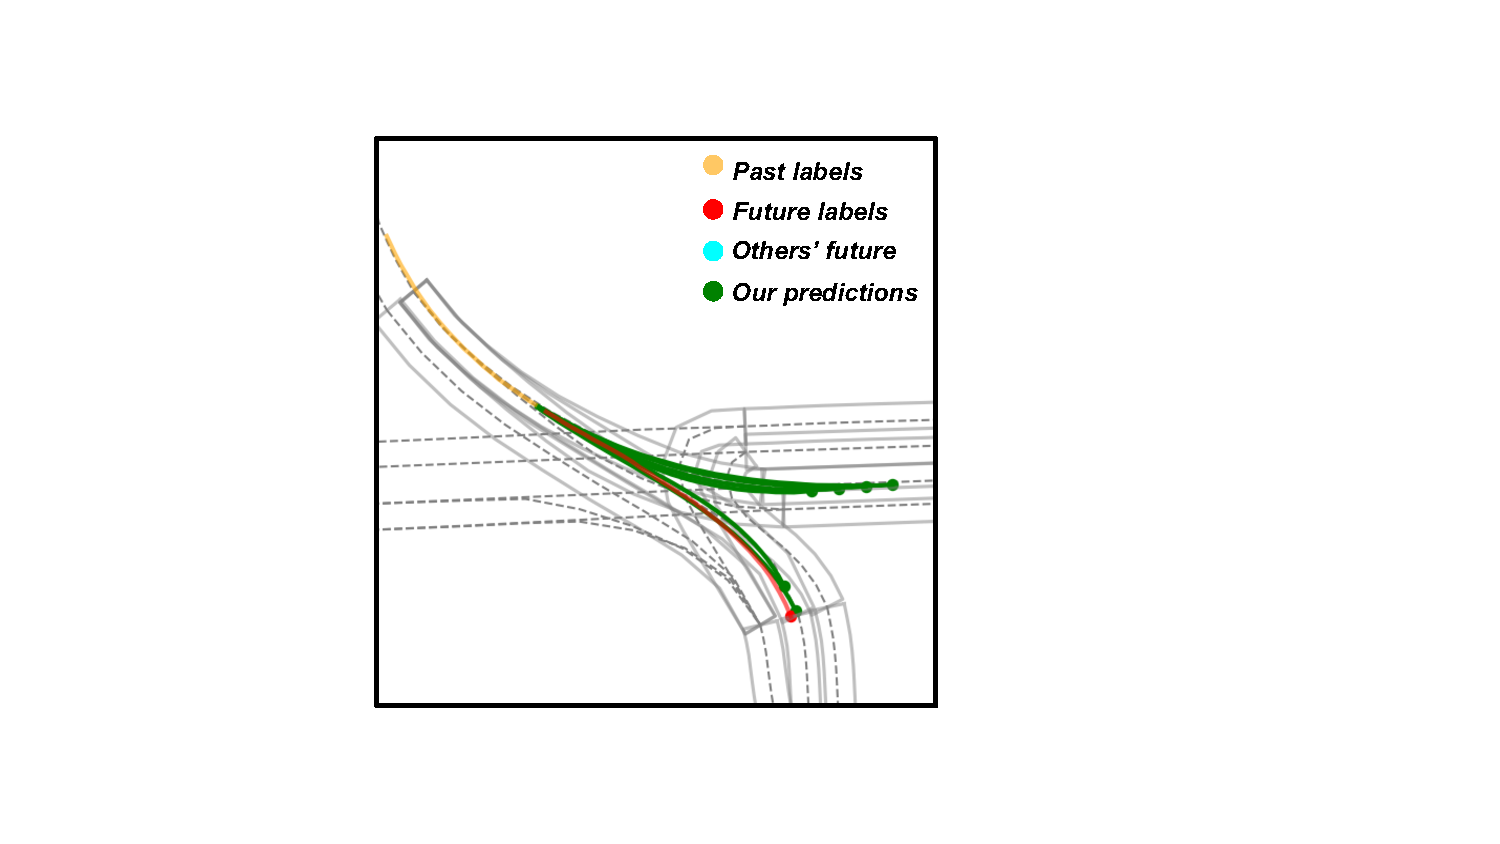
\includegraphics[width=0.24\linewidth]{figures/vis1.pdf}
&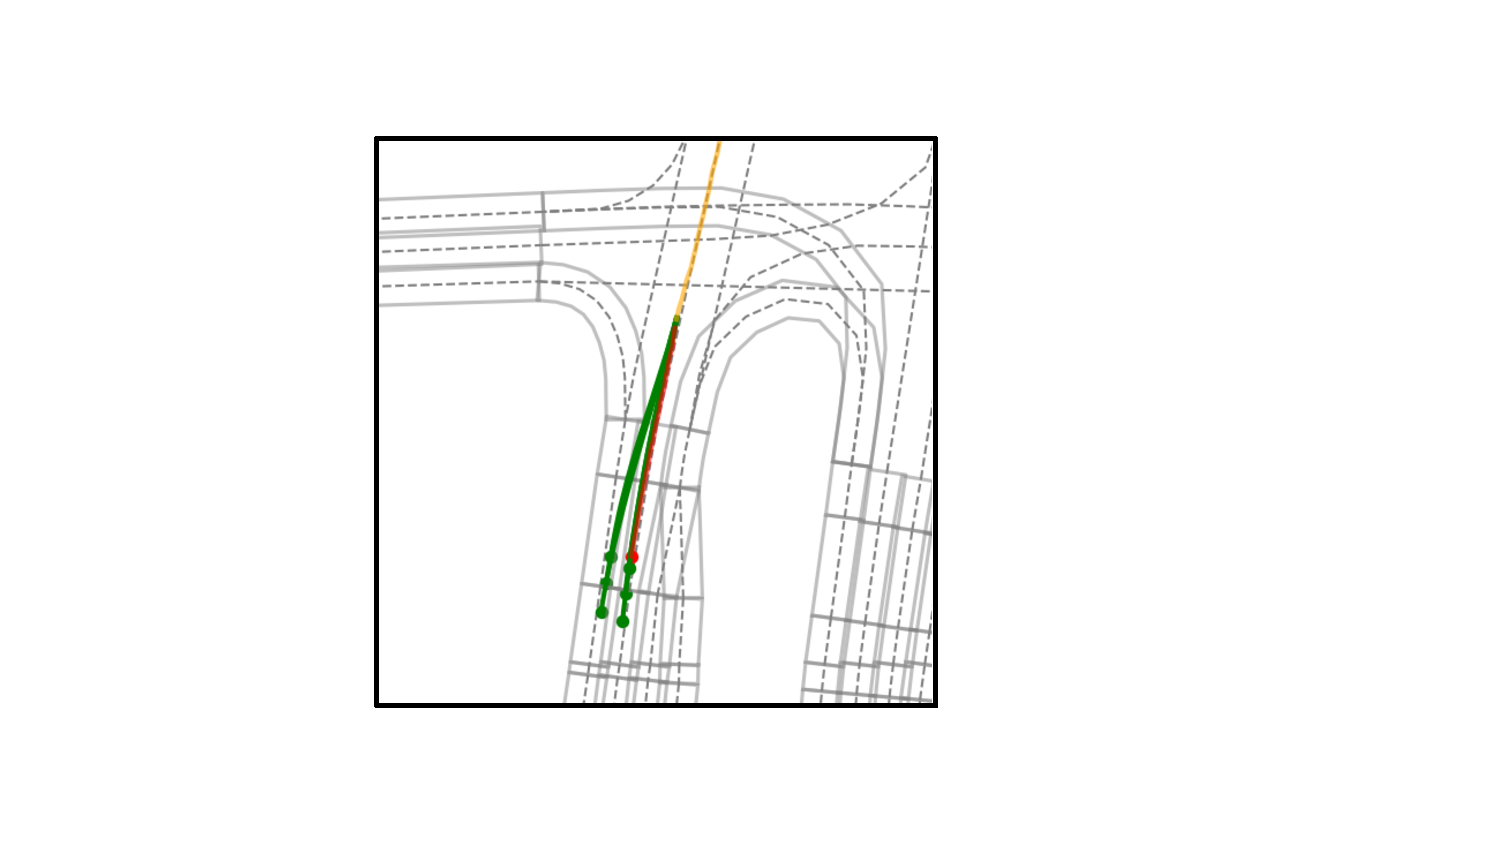
\includegraphics[width=0.24\linewidth]{figures/vis2.pdf}
&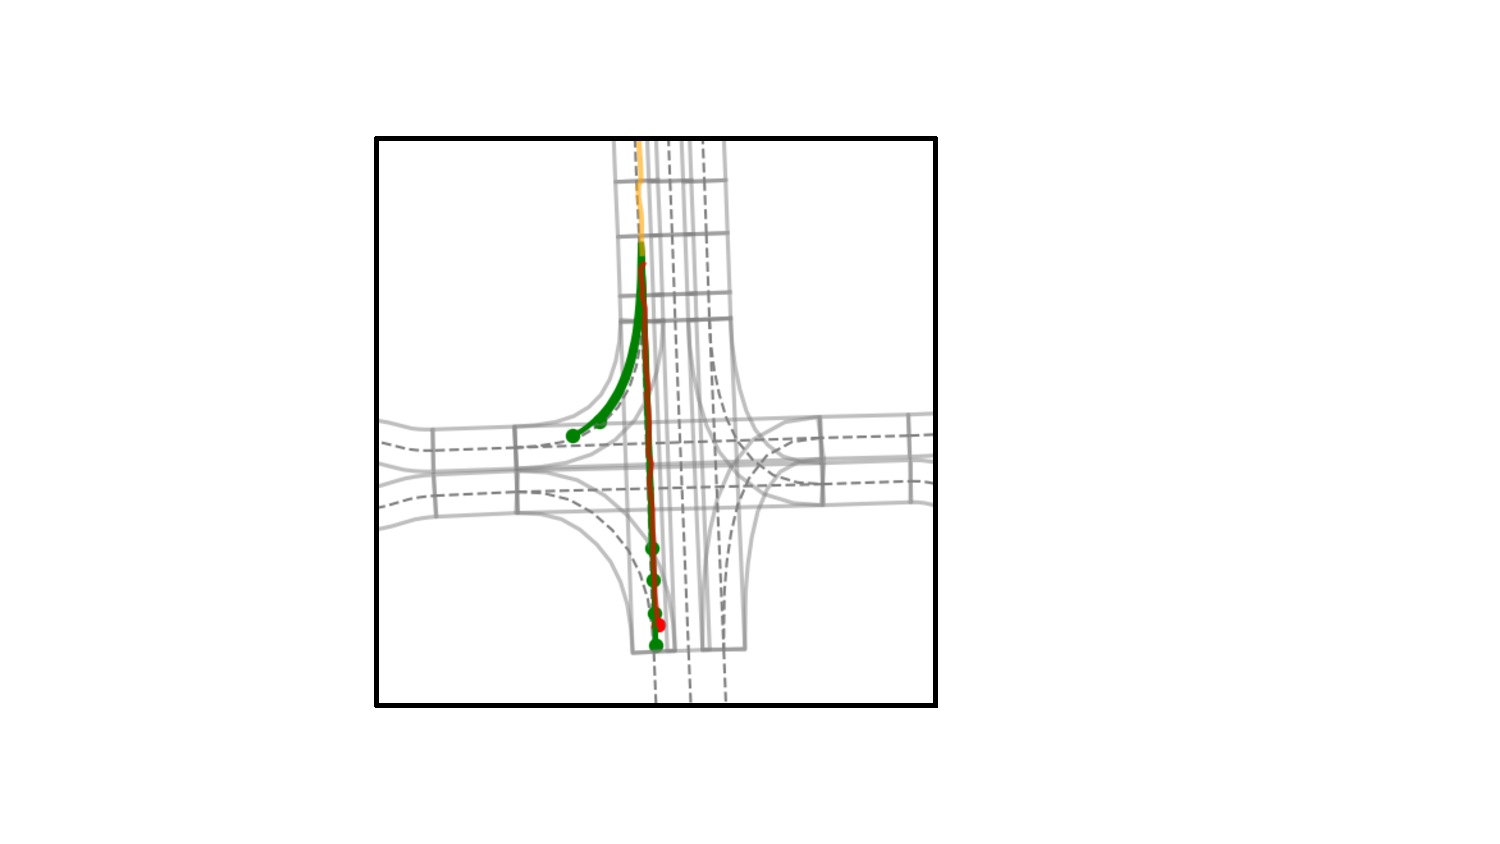
\includegraphics[width=0.24\linewidth]{figures/vis3.pdf}
&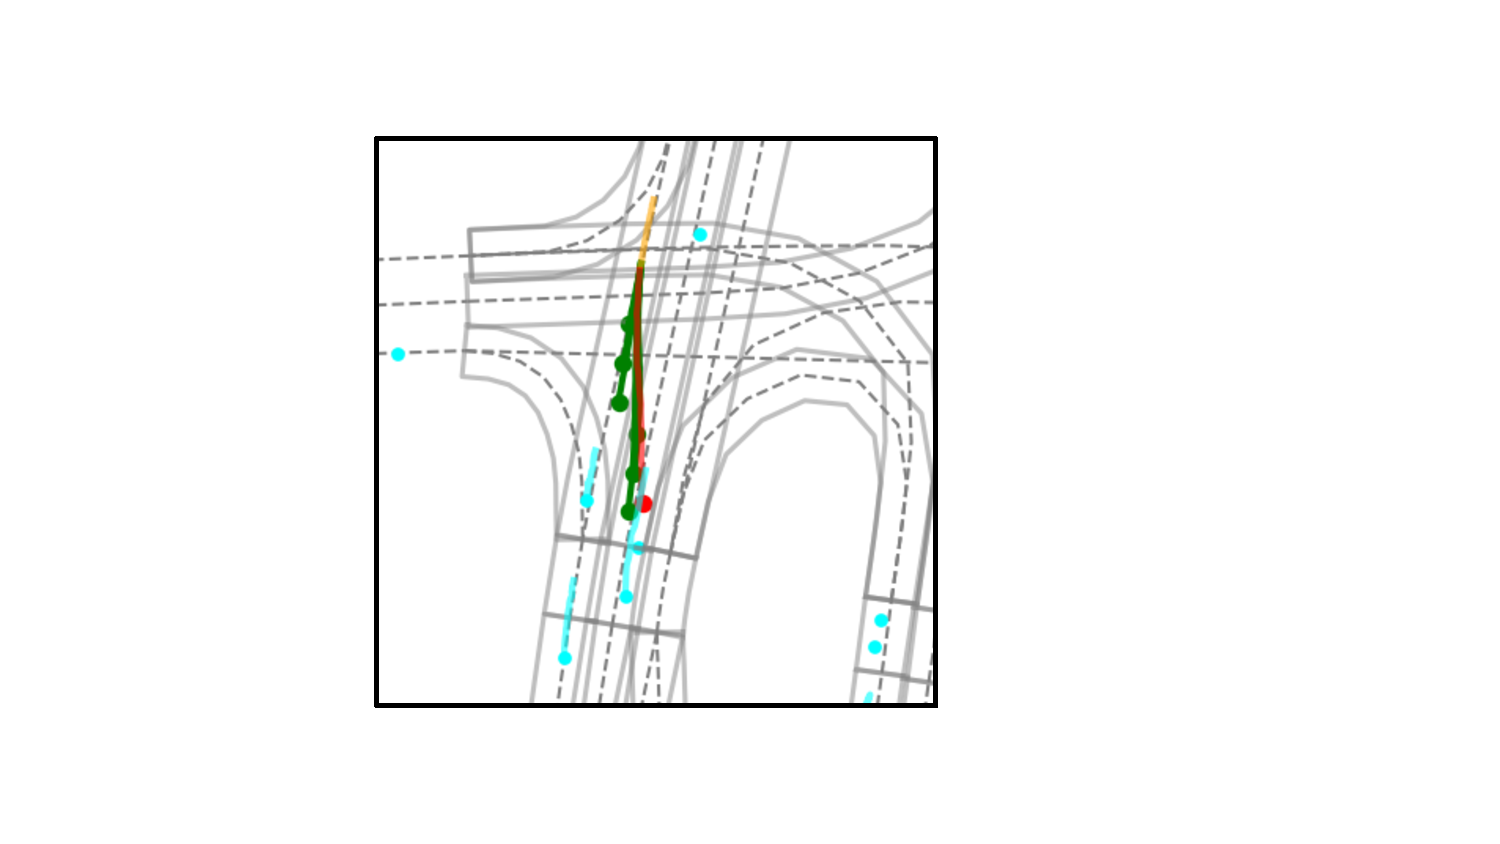
\includegraphics[width=0.24\linewidth]{figures/vis4.pdf}

\end{tabular}
\caption{Qualitative results on Argoverse validation set. Here we show (from
left-to-right): 1) curved lanes 2) lane changing 3) intersection 4) overtaking.}
\label{fig:vis}
\vspace{-0.2cm}
\end{figure*}

\subsection{Ablation Studies}





\paragraph{Ablations on LaneRoI Encoder}
We first show the ablation study on one of our main contributions, \ie, \ROI, in the upper half of Table
\ref{table:ablation}. 
The first row shows a representative of the traditional representations. 
Specifically, we first build
embeddings for lane graph nodes using only the map information and 4 lane
convolution layers. We then use a
1D CNN (U-net style) to extract a motion feature vector from actor kinematic states, concatenate it
with every graph node embedding and make predictions. Conceptually, this is
similar to TNT \cite{tnt} except that we modify the backbone network to make comparisons fair. 
On the second row, we show the result of our \ROI
representations with again four lane convolution layers (no shortcuts). Hence, the only difference
is whether the actor is encoded with a single motion vector shared by
all nodes, or encoded in a distributed and structured manner as ours. As shown
in the table, our \ROI achieves similar or better results on all
metrics, exhibiting its advantages. Note that this row is not yet our best result
in terms of using \ROI representations, as the actor information is only exposed
to a small region during the input encoding (clamping at input
node embeddings) and can not efficiently propagate to
the full \ROI without the help of the shortcut, which we will show next.

Subsequent rows in Table \ref{table:ablation} compare different design
choices for the shortcut mechanism, in particular how we pool the global feature
for each \textit{LaneRoI}. `Global Pool' refers to average-pooling all node
embeddings within a \textit{LaneRoI}, and `Center Pool' means we pool a feature
from a \ROI using nodes that around the last observation of the actor and a lane
pooling. As we can see, although these two approaches can possibly
spread out information to every node in a \textit{LaneRoI} (and thus build a
shortcut), they barely improve the performance. On the contrary, ours achieve
significant improvements. This is because we pool features along the past
trajectory of the actor, which results in a larger and actor-motion-specific receptive field.
Here, $\times 1$ and $\times 2$ refer to an encoder with 1 shortcut per 4 and 2 lane
convolution layers respectively. This shows stacking more shortcuts
provides some, but diminishing, benefits.









\paragraph{Ablations on LaneRoI Interactor}
To verify the effectiveness of our map-aware interaction module, we compare against several model variants based
on the fully-connected interaction graph among actors. Specifically, for each actor,
we apply a \ROI encoder\footnote{We choose \ROI encoder rather than other
encoder, \eg, CNN, for fair comparisons with ours.} to process node embeddings, and then pool an
actor-specific feature vector from \ROI via either the global average pooling or our
shortcut mechanism. These actor features are then fed into a transformer-style
\cite{transformer} attention module or a fully-connected GNN.
Finally, we add the output actor features to nodes in their \ROI respectively
and make predictions using our decoding module.
As a result, these variants have the same pipeline as ours, with the only
difference on how to communicate across actors. To make comparisons
as fair as possible, both the attention and GNN have the same
numbers of layers and channels as our \ROI Interactor.\footnote{The GNN here is almost identical to our lane
convolution used in Interactor except for removing the multi-hop as the graph is fully-connected.}

As shown in Table \ref{table:ablation}, all interaction-based models outperform
the one without considering interactions (row 1) as expected. In addition, our
approach significantly improves the performance compared to both the attention and GNN. 
Interestingly, all fully-connected interaction graph based model reach similar
performance, which might imply such backbones may saturate the performance (as
also shown by leading methods on the leaderboard).
We also show that naively using the average pooling to embed features from
\textit{LaneRoI}s to global graph does not achieves good performance
because it ignores local structures.

\subsection{Qualitative results}
In Figure~\ref{fig:vis}, we show some qualitative results on Argoverse validation
set. We can see that our method generally follows the map very well and demonstrates good
multi-modalities. From left to right, we show 1) when an actor follows a
curved lane, we predict two direction modes with different velocities;
2) when it is on a straight lane, our model covers the possibilities of lane changing; 3)
when it's approaching an intersection, our model captures both the go-straight and the
turn-right modes, especially with lower speeds for turning right, which are
quite common in the real world; 4) when there is an actor blocking the path, we
predict overtaking behaviors matching exactly with the ground-truth. Moreover,
for the lane-following mode, we predict much slower speeds which are consistent with
this scenario, showing the effectiveness of our interaction modeling. 
% We provide more qualitative results in the supplementary~\ref{sec:supp_qual}.



\section{Conclusion}

In this paper, we propose LaneRCNN, a graph-centric motion forecasting model.
Relying on learnable graph operators, LaneRCNN builds a distributed lane-graph-based
representation (\textit{LaneROI}) per actor to encode its past motion and the local map topology.
Moreover, we propose an interaction module which effectively captures the interactions among actors within the shared global lane graph.
And lastly, we parameterize the output trajectory using lane graphs which helps improve the prediction.
We demonstrate that LaneRCNN achieves state-of-the-art performance on the challenging Argoverse motion forecasting benchmark.

% 
\section*{Acknowledgement}
We would like to sincerely thank Siva Manivasagam, Yun Chen, Bin Yang, Wei-Chiu Ma and
Shenlong Wang for their valuable help on this paper.



%%%%%%%%%%%%%%%%%%%%%%%%%%%%%%%%%%%%%%%%%%%%%%%%%%%%%%%%%%%%%%%%%%%%%%%%%%%%%%%%

%%%%%%%%%%%%%%%%%%%%%%%%%%%%%%%%%%%%%%%%%%%%%%%%%%%%%%%%%%%%%%%%%%%%%%%%%%%%%%%%
% \section*{APPENDIX}
% Appendixes should appear before the acknowledgment.
% \section*{ACKNOWLEDGMENT}




%%%%%%%%%%%%%%%%%%%%%%%%%%%%%%%%%%%%%%%%%%%%%%%%%%%%%%%%%%%%%%%%%%%%%%%%%%%%%%%%



\bibliographystyle{IEEEtran}
\bibliography{mybib}





\end{document}
